\begin{figure}[H]
  \centering
  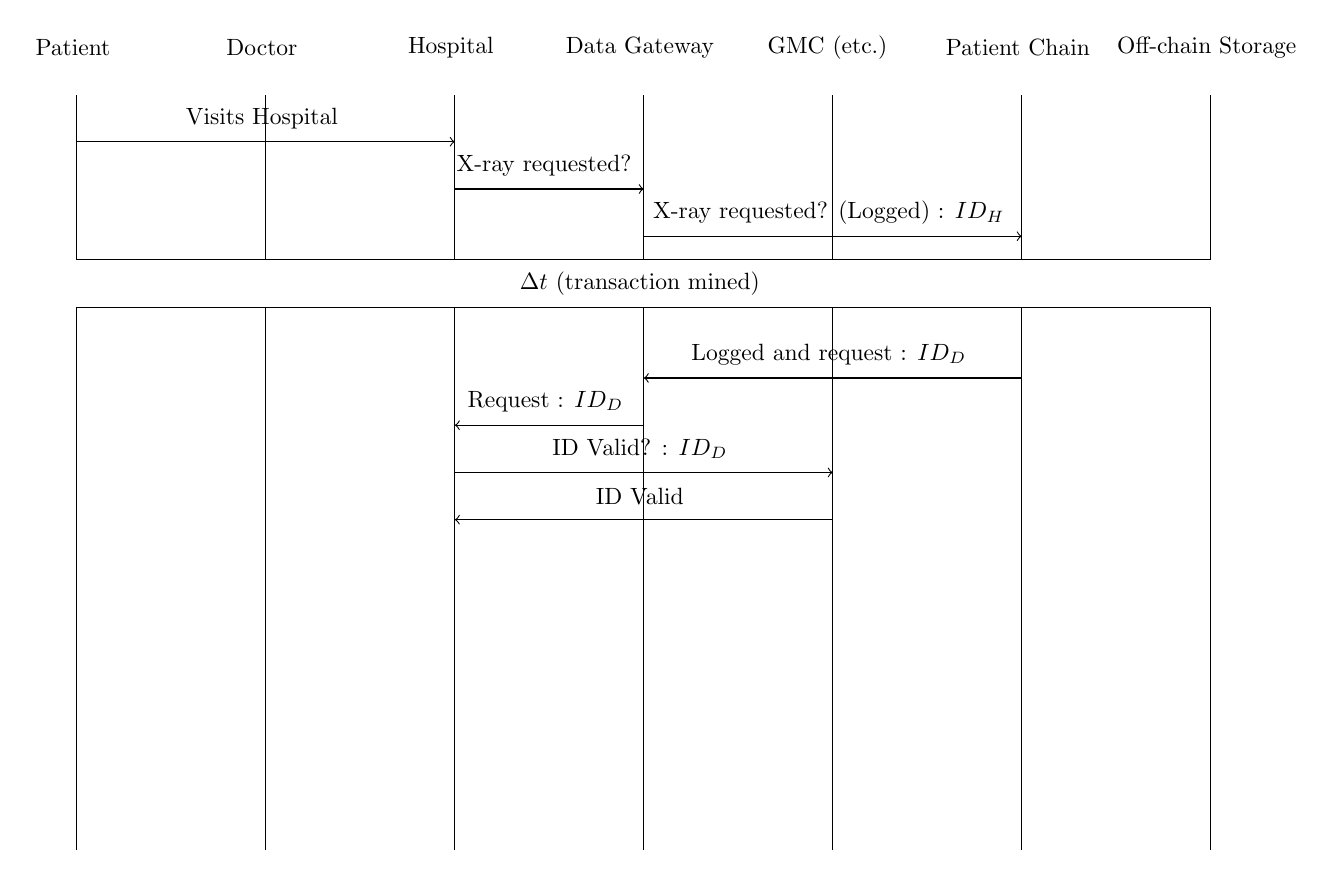
\begin{tikzpicture}[scale = 0.6, every node/.style={scale = 0.85}]

  % Lines
  \draw (4, 4) -- (4, 15.5);
  \draw (4, 16.5) -- (4, 20);
  \draw (8, 4) -- (8, 15.5);
  \draw (8, 16.5) -- (8, 20);
  \draw (12, 4) -- (12, 15.5);
  \draw (12, 16.5) -- (12, 20);
  \draw (16, 4) -- (16, 15.5);
  \draw (16, 16.5) -- (16, 20);
  \draw (20, 4) -- (20, 15.5);
  \draw (20, 16.5) -- (20, 20);
  \draw (24, 4) -- (24, 15.5);
  \draw (24, 16.5) -- (24, 20);
  \draw (28, 4) -- (28, 15.5);
  \draw (28, 16.5) -- (28, 20);

  % Headings
  \node[align = center] at (4, 21) { Patient };
  \node[align = center] at (8, 21) { Doctor };
  \node[align = center] at (12, 21) { Hospital };
  \node[align = center] at (16, 21) { Data Gateway };
  \node[align = center] at (20, 21) { GMC (etc.) };
  \node[align = center] at (24, 21) { Patient Chain };
  \node[align = center] at (28, 21) { Off-chain Storage };

  % Arrows
  \node[align = center] at (8, 19.5) { Visits Hospital };
  \draw [ -> ] (4, 19) -- (12, 19);

  \node[align = center] at (14, 18.5) { X-ray requested? };
  \draw [ -> ] (12, 18) -- (16, 18);

  \node[align = center] at (20, 17.5) { X-ray requested? (Logged) : $ID_{H}$ };
  \draw [ -> ] (16, 17) -- (24, 17);

  \draw (4, 16.5) -- (28, 16.5);
  \node[align = center] at (16, 16) { $\Delta t$ (transaction mined) };
  \draw (4, 15.5) -- (28, 15.5);

  \node[align = center] at (20, 14.5) { Logged \checkmark and request : $ID_{D}$ };
  \draw [ -> ] (24, 14) -- (16, 14);

  \node[align = center] at (14, 13.5) { Request : $ID_{D}$ };
  \draw [ -> ] (16, 13) -- (12, 13);

  \node[align = center] at (16, 12.5) { ID Valid? : $ID_{D}$ };
  \draw [ -> ] (12, 12) -- (20, 12);

  \node[align = center] at (16, 11.5) { ID Valid \checkmark };
  \draw [ -> ] (20, 11) -- (12, 11);

  

  \end{tikzpicture}
  \caption{
    Patient visits hospital to have X-ray taken
  }
  \label{fig:user_story_02}
\end{figure}
